\subsection{Высокоуровневый обзор}
Высокоуровневое архитектурное представление cистемы сфокусировано на взаимодействии с пользователями и потоке данных, связанных с данными, отправляемыми пользователями.

\textbf{Управление пользователями:}
\noindent
\begin{itemize}
    \itemsep 0em
    \item Пользователи регистрируются в системе, предоставляя основную информацию, такую как имя пользователя и электронная почта. Дополнительные сведения о профиле, такие как имя, местоположение и принадлежность, фиксируются в отдельной таблице.
   \item Система сможет различать роли пользователей с помощью флагов (is\_staff), что позволяет использовать механизмы гранулярного контроля доступа.
\end{itemize}

\textbf{Обработка решений:}
\noindent
\begin{itemize}
    \itemsep 0em
    \item Пользователи отправляют данные по установленным каналам, и система записывает ссылку на исходный код и временную метку отправки для каждого экземпляра.
    \item Центральная система очередей, работающая на базе Celery, эффективно управляет обработкой поступающих решений, обеспечивая оптимальное использование ресурсов.
    \item Предоставленные данные надежно хранятся в облачном хранилище, используя его масштабируемость и гибкость для работы с различными форматами данных.
\end{itemize}

\textbf{Сохранение данных:}
\noindent
\begin{itemize}
\itemsep 0em
    \item Данные о пользователях, включая информацию о профиле и историю активности, хранятся в базе данных MySQL. Эта реляционная структура базы данных позволяет эффективно выполнять запросы и управлять структурированными данными.
    \item Данные об отправке решений хранятся в базе данных MongoDB, что позволяет использовать ее масштабируемость и гибкость при работе с потенциально большими и неоднородными форматами данных.
\end{itemize}

% \subsection{Балансировка нагрузки}

% \subsection{Мониторинг}



\subsection{Обзор пути обработки решений}
\begin{figure}[h]
    \centering
    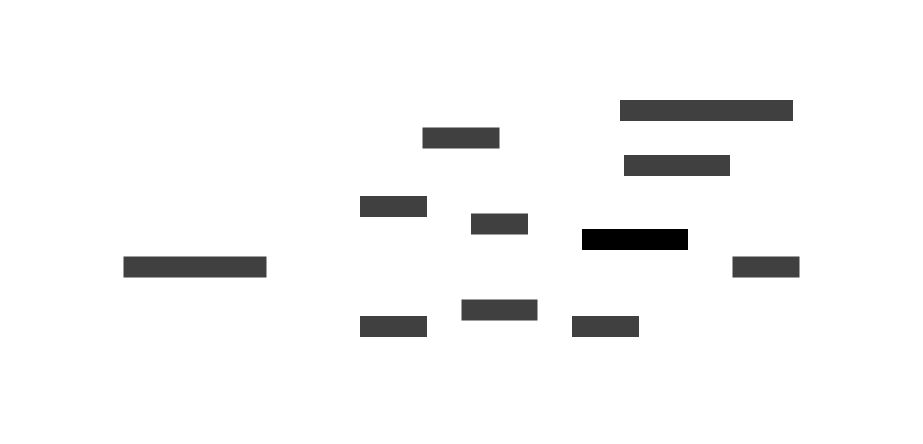
\includegraphics[width=0.8\textwidth]{submission_process.png}
    \caption{Путь обработки решения}
\end{figure}

\subsubsection{Выбор контайнера и распределенное выполнение}
% Выбор контайнера в данном интерфейсе производится 

\subsubsection{Выполнение тестов и возврат вердиктов}

\subsubsection{Агрегация и хранение вердиктов}

\subsubsection{Трейсинг в реальном времени}

